\section*{Problem 5}

$x(t)=e^{-3t}cos(10t)u(t)$

\subsection*{Solution}

From the 1st result of the Fourier Transforms table we have:

\begin{equation}
\mathfrak{F}\{ e^{-\alpha t} u(t)\} = \frac{1}{\alpha + j \omega} 
\label{eq:c2p5}
\end{equation} 

Rearranging the equation for $x(t)$ we have:

\begin{equation*}
\begin{aligned}
x(t) &= \frac{1}{2} [e^{-3t}e^{10 j t} + e^{-3t}e^{-10 j t}] u(t) \\
     &= \frac{1}{2} [e^{-t(3 - 10j)} + e^{-t(3 + 10j)}] u(t)
\end{aligned}
\end{equation*} 

We can now apply directly the result from (\ref{eq:c2p5}):

\begin{equation*}
\begin{aligned}
X(\omega) &=  \frac{1}{2} \left[
	\frac{1}{(3 - 10j) + j\omega} + 
	\frac{1}{(3 + 10j) + j\omega} \right] \\
          &=  \frac{1}{2} \left[
	\frac{1}{3 + (\omega - 10)j } + 
	\frac{1}{3 + (\omega + 10)j} \right] \\
\end{aligned}
\end{equation*} 

The plot of the magintude of $X(\omega)$ is:
\zcodemat{sources/c2p5.m}{Plot of Magnitude}

\begin{figure}[H]
\caption{Magnitude $|X(\omega)|$}
\centering
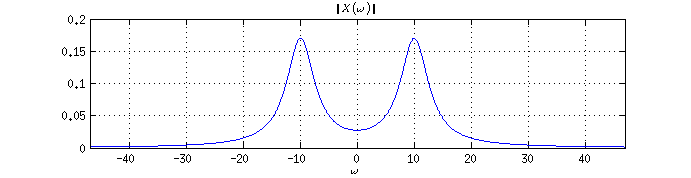
\includegraphics[width=1.0\textwidth]{figs/c2p5a.png}
\label{fig:c2p5a}
\end{figure} 

